\section{Замеры}

\subsection{$U = 1$}
Для вычислений я сгенерировал по 100 реплик длины 250, 500, 1000, 2000. При моделировании методом Монте-Карло делал 100000--300000 шагов на отжиг, и 500000--1000000 шагов для замеров. 
Оказалось что достаточно большая часть этих конформаций неплотные, то есть их свойства ближе к свойствам одномерной решётки, чем двумерной. При попытке посчитать среднее значения кумулянта Биндера неплотные конформации Сильно влияли на значение кумулянта, увеличивая погрешность от реплики к реплике.

\begin{figure}[h]
	\centering
	\begin{subfigure}[t]{0.48\textwidth}
		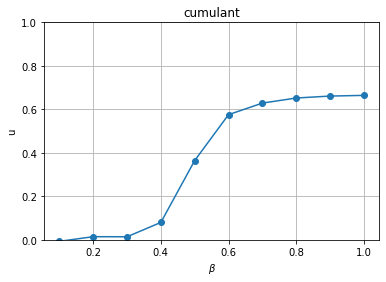
\includegraphics[width=\textwidth]{../images/dense_cumulant.png} 
		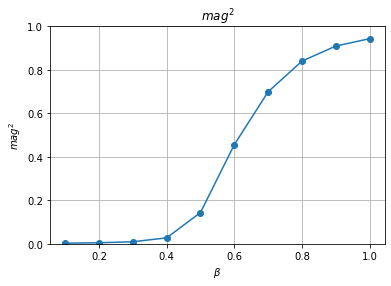
\includegraphics[width=\textwidth]{../images/dense_magnetization.png} 
		\caption{Плотная}
	\end{subfigure}
	\begin{subfigure}[t]{0.48\textwidth}
		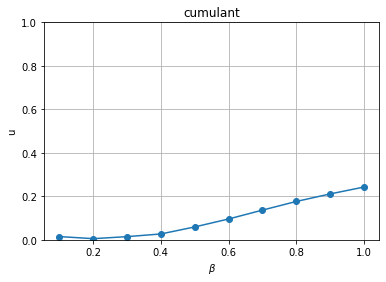
\includegraphics[width=\textwidth]{../images/loose_cumulant.png} 
		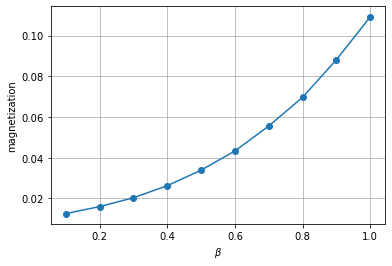
\includegraphics[width=\textwidth]{../images/loose_magnetization.png} 
		\caption{Неплотная}
	\end{subfigure}
	\caption{Пример кумулянта и намагниченности плотной и неплотной конформаций}
\end{figure}


Для определения "плотности" реплики вычисляется её радиус инерции $R = \sqrt{\frac{1}{n}\sum_{i=1}^{n}r_{i}^{2}}$, где $r_i$ это расстояние от узла конформации до её центра масс. Реплики размера 250, 500, 1000, 2000 отбрасываются если их радиусы больше 7.7, 13.5, 18, 25 соответственно, доля отброшенных реплик 0.54, 0.35, 0.37, 0.47 соответственно. Для размеров 500, 1000, 2000 я подбирал радиусы для разделения по значению кумулянта при $\beta = 1$ (рис. \ref{fig:cumul_cor}), для 250 я так же ориентировался на значение намагниченности при $\beta = 1$ (рис. \ref{fig:L250_mag_cor}). Вместо радиусов удобнее использовать значение, вычисляемое по формуле $R/\sqrt{L}$. Радиусам 7.7, 13.5, 18, 25 и длинам конформаций 250, 500, 1000, 2000 соответствуют значения 0.49, 0.6, 0.57, 0.56.

\begin{figure}[h]
	\centering
	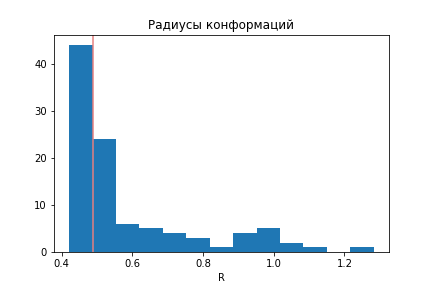
\includegraphics[width=0.48\textwidth]{../images/R_hist_L250.png} 
	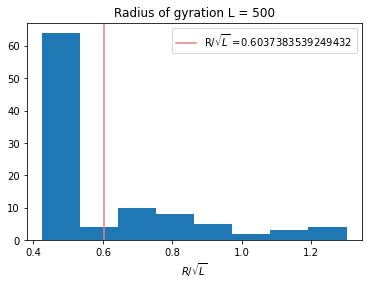
\includegraphics[width=0.48\textwidth]{../images/R_hist_L500.png} 
	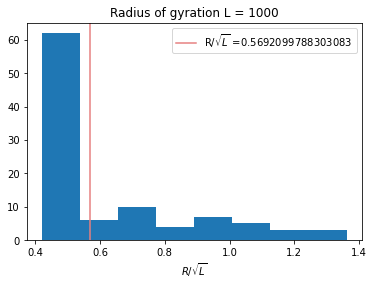
\includegraphics[width=0.48\textwidth]{../images/R_hist_L1000.png} 
	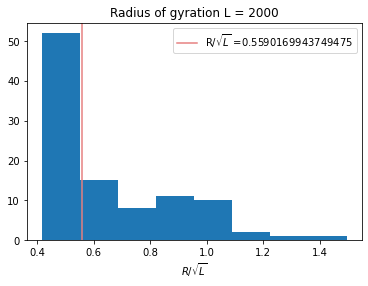
\includegraphics[width=0.48\textwidth]{../images/R_hist_L2000.png} 
	\caption{Гистограммы радиусов полей размеров 250, 500, 1000, 2000}
\end{figure}

\begin{figure}[h]
	\centering
	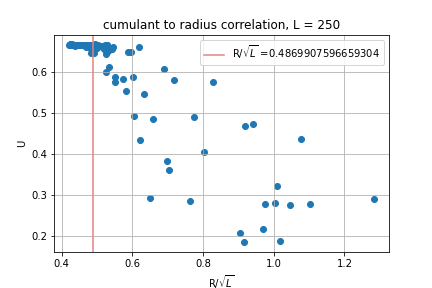
\includegraphics[width=0.48\textwidth]{../images/cumulant_to_R_L250.png} 
	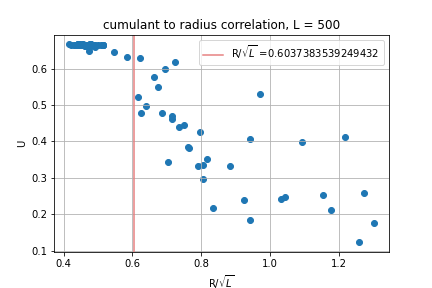
\includegraphics[width=0.48\textwidth]{../images/cumulant_to_R_L500.png} 
	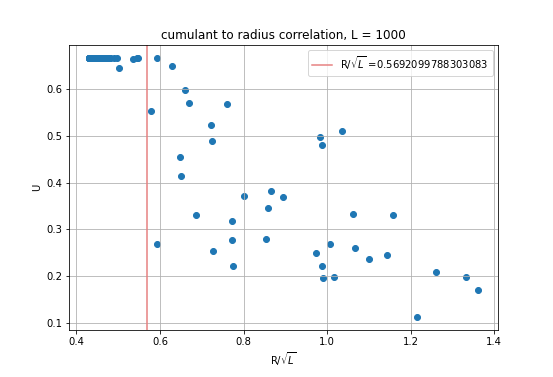
\includegraphics[width=0.48\textwidth]{../images/cumulant_to_R_L1000.png} 
	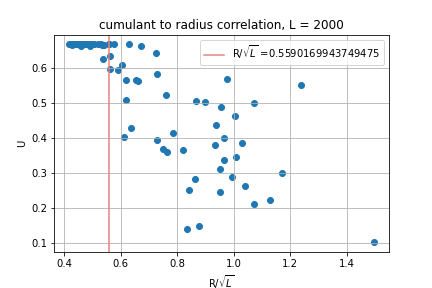
\includegraphics[width=0.48\textwidth]{../images/cumulant_to_R_L2000.png} 
	\label{fig:cumul_cor}
	\caption{Корреляция радиусов со значением кумулянта, красными линиями отмечены радиусы по которым отбрасываются конформации(7.7, 13.5, 18, 25)}
\end{figure}

\begin{figure}[h]
	\centering
	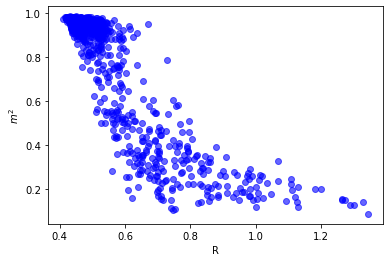
\includegraphics[width=1\textwidth]{../images/mag2_to_R_L250.png} 
	\caption{Корреляция радиусов с квадратом намагниченности, красными линиями отмечены радиусы по которым отбрасываются конформации}
	\label{fig:L250_mag_cor}
\end{figure}


Кумулянт Биндера для одной реплики при заданной температуре вычисляется по формуле $U = 1 - \frac{\langle m^4\rangle}{3\langle m^2\rangle ^2}$. Дальше Значения усредняются между репликами при каждой температуре $\langle U\rangle = \frac{1}{n}\sum_{i=1}^{n}U_i$ 
Погрешность кумулянта от реплики к реплике вычисляется как среднеквадратичное отклонение по формуле $\sqrt{\frac{1}{n}\sum_{i=1}^{n}(\langle U\rangle - U_i)^2}$


\begin{figure}[h]
	\centering
	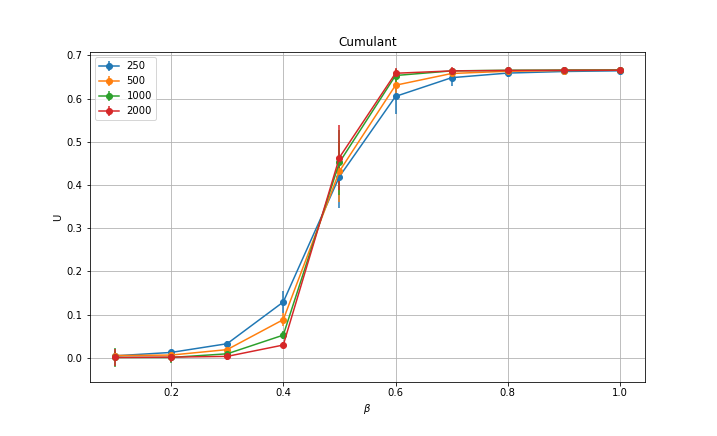
\includegraphics[width=1\textwidth]{../images/Cumulant_big.png} 
	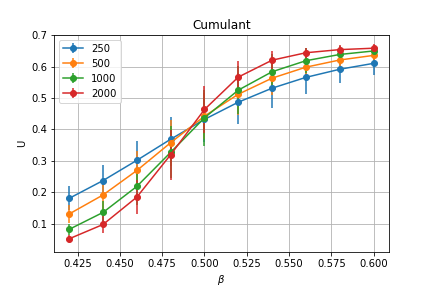
\includegraphics[width=1\textwidth]{../images/Cumulant_beta0.4_0.6.png} 
	\caption{Значения куулянтов после отбрасывания конформаций по радиусам}
\end{figure}
